% !TEX root = thesis.tex

%%
%%
%% Merged Literature and Theoretical Background chapter
%%
%%

Our research is concerned with two-dimensional non-parametric intensity estimation,
that is estimating functions in the plane while making only minimal assumptions about the underlying distribution of the data. 
This technique has been applied in several areas of spatial analysis including epidemiology.
In particular, we are interested in estimating the \textit{\gls{risk}} of developing a disease.
In order to be precise, we define
\begin{defn}
    \textbf{\Gls{risk}} is the probability of an individual person contracting a disease in a specific time period
    \citet[Chapter 2]{rothman2008modern}.
\end{defn}

%%%%%%%%%%%%%%%%%%%%%%%%%%%%%%%%%%%%%%%%%%%%%%%%%%%%%%%%%%%%%%%%%%%%%%%%%%%%%%
%%
%% Disease incidence
%%
%%%%%%%%%%%%%%%%%%%%%%%%%%%%%%%%%%%%%%%%%%%%%%%%%%%%%%%%%%%%%%%%%%%%%%%%%%%%%%
\section{Disease incidence}
\label{sec:theory:incidence}

The theory described in this section is based on \citet{rothman2008modern}.
We focus on chronic diseases in order to better understand the degree to which different groups of people are ``at risk'' of contracting a disease.
We also are interested in discovering and describing the association between environmental factors and this ``risk''.
For example, one could ask if air pollution emitted by a factory is associated with an increased ``risk'' of lung cancer among people that live close by.

In order to be more precise, let us define

\begin{defn}
    \textbf{\Gls{risk}} is the probability of an individual person contracting a disease in a specific time period.
\end{defn}

One way to estimate the \gls{risk} is to look at the historical frequency of contracting of the disease.
The type of study we are interested in involves incidents of a chronic disease.
Therefore, we separately consider those people who contracted the disease under study.
In particular, we are interested in people who did not have the disease at the beginning of the study,
but developed the disease within the study period.
These are new cases of the disease, which we call \textbf{\glspl{incident}}.

\begin{defn}
    An \textbf{\gls{incident}} is a new case of the disease during the study period.
\end{defn}

The common measure of frequency used in the literature compares the number of new cases of a disease to the total time spent by members of the population in the study.
This measure is called the \gls{incidence rate}.

\begin{equation}
    \mbox{\Gls{incidence rate} (common definition)} = \frac{\mbox{number of new cases}}
                                {\displaystyle\smashoperator{\sum\limits_{\mbox{persons}}}\mbox{time spent by person in population}}
\end{equation}

For our simulation study, we can simplify our definition of \gls{incidence rate} by assuming that each person in the population is exposed for the entire study period,
which for simplicity we can set to one (1).
Our simplified definition of incidence rate is then:

\begin{defn}
    The \textbf{\gls{incidence rate}} is the number of new cases in the study period divided by the total population.
    \begin{equation}
        \label{eq:incidencerate}
        \mbox{\Gls{incidence rate}} = \frac{\mbox{number of new cases in a time period}}
                                        {\mbox{number of persons}}
    \end{equation}
\end{defn}

\Glspl{incidence rate} are always expressed in cases per person-time units.
For example, 10 cases of asthma per 100,000 people per year is a valid \gls{incidence rate}.

For a given population, time period, and set of \glspl{incident},
we can compute the overall \gls{incidence rate} by taking the total number of \glspl{incident} and dividing by the total population.
However, we may wish to compare the \gls{incidence rate} at different locations within an area.
To do this, we need to look at the number of cases and the population in the areas that are close to these locations.
If we then make these areas infinitesimally small,
then we could compute the \gls{incidence rate} point-wise.

\begin{defn}
    \label{defn:incidence_rate}
    The \textbf{point-wise \gls{incidence rate}} is a function that computes the local \gls{incidence rate} at a point by dividing the point-wise value of the number of new cases by the point-wise value of the population.
\end{defn}

From this point onwards, the term \gls{incidence rate} refers to the point-wise \gls{incidence rate}.

%%%%%%%%%%%%%%%%%%%%%%%%%%%%%%%%%%%%%%%%%%%%%%%%%%%%%%%%%%%%%%%%%%%%%%%%%%%%%%
%%
%% Spatial point processes
%%
%%%%%%%%%%%%%%%%%%%%%%%%%%%%%%%%%%%%%%%%%%%%%%%%%%%%%%%%%%%%%%%%%%%%%%%%%%%%%%
\section{Spatial point processes}
\label{sec:theory:spatial_point_processes}

The estimation of intensity is part of the wider field of spatial pattern analysis.
For event data such as disease incidence,
spatial point processes including Poisson processes are often used to model
the statistical and spatial properties of events.
\Citet{diggle1983spatial} is an early publication which extensively covers
the spatial-statistical analysis of point patterns such as these.
It covers several stochastic models and statistical methods,
and provides examples of biological and epidemiological analyses.

\begin{color}{red}
The theoretical results in this section are taken from \citet{diggle1983spatial},
\citet{diggle1988equivalence},
\citet{guan2008consistent},
\citet{silverman1986density},
and \citet{wand1994kernel}.
\end{color}

In order to understand the geospatial patterns of disease incidence,
we consider points in two-dimensional space $\RS$.
We begin with

\begin{defn}
    \label{defn:studyarea}
    A \textbf{study area} $\gls{W} \subset \RS$ is a region in the plane where we make observations.
\end{defn}

The observations we are interested in are points distributed in \gls{W} which we call \textbf{events}.

\begin{defn}
    \label{defn:event}
    An \textbf{event} is a point $\xvec \in \RS$, situated in a study area \gls{W} that we are interested in observing.
\end{defn}

For example, in the study area of the boundaries of a city, we consider the events of the addresses of the residents.
We call this set of events

\begin{defn}
    The \textbf{population} \gls{P} is the set of home address events of the residents of the study area \gls{W}.
\end{defn}

In general, we are interested in understanding the mechanism by which the events occurred.
We are interested both in the number of events, and even more so in the pattern by which their locations are distributed in \gls{W}.
Taking a spatial statistical approach, we model the underlying mechanism that generates events using the following:

\begin{defn}
    \label{defn:spp}
    A \textbf{\gls{spp}} $\boldsymbol{\gls{Lambda}}$ is a stochastic mechanism which generates a random set of events.
\end{defn}

Suppose we have a \gls{spp} \gls{Lambda} on a study area $\gls{W} \subset \RS$.
We can count the total number of \glspl{event} and divide it by the total area of \gls{W}.
This gives us a quantity we call the \textbf{average \gls{intensity}} of \gls{Lambda}.
Sometimes the points are spread uniformly throughout \gls{W}.
In that case, we say that \gls{Lambda} is a homogeneous point process.
On the other hand, it is often the case that \gls{Lambda} is not uniform,
and we call it a heterogeneous point process.
When \gls{Lambda} is heterogeneous,
we would like to know the average \gls{intensity} around different points in \gls{W}.
For this
we define $\ds$ as an infinitesimal area around the point $\xvec$,
and $N\!(\ds)$ as the number of \glspl{event} inside $\ds$.
Then the \textbf{\gls{intensity}} $\boldsymbol{\gls{lambda}\xvec}$ at $\xvec \in \RS$ is

\begin{equation}
    \label{eq:lambda_differential}
    \lambda \xvec := \lim_{|\ds| \to 0}
        \left\{
            \frac{\mathbb{E}[N\!(\ds)]}% /
            {|\ds|}
        \right\}
\end{equation}

We model disease incidence as a special kind of \gls{spp} known as an Inhomogeneous Poisson Process.
\begin{defn}
    \label{defn:inhomogenouspoissonprocess}
    An \textbf{Inhomogeneous Poisson Process} is a \gls{spp} which has the following properties \citep[Section 4.4]{diggle1983spatial}:
    \begin{properties}
        \item The number of events $N\!(A)$ in any area $A$ has a Poisson distribution with mean
            $\iint\limits_{\xvec \in A}{\hspace{-1em} \lambda \xvec \diff{x_2} \diff{x_1}}$
            \label{defn:inhomogenouspoissonprocess:1}.
        \item Conditioning on $N\!(A) \! = \! n$,
            the $n$ events (locations) in $A$ form an independent random sample from the distribution on $A$ with probability density function \textit{proportional} to $\lambda$ \label{defn:inhomogenouspoissonprocess:2}.
    \end{properties}
\end{defn}

From above, we can see that for an infinitesimal area \ds~ around a point \xvec,
we can think of $\lambda \xvec \ds$ as nearly constant in \ds~so
$$\iint\limits_{\xvec \in A}{\hspace{-1em}\lambda \xvec \diff{x_2} \diff{x_1}} \approx \lambda \xvec \ds \text{.}$$
By \cref{defn:inhomogenouspoissonprocess:1} of \Cref{defn:inhomogenouspoissonprocess},
the probability that the are \ds~ contains exactly one point is
$\exp(-\lambda \xvec |\!\ds|) \lambda \xvec \ds \text{.}$
Since we take \ds~ to be infinitesimal,
$\exp(-\lambda \xvec |\!\ds|) \allowbreak \approx 1$ and so we can think of
$\lambda \xvec \ds$ as the probability that \ds~ contains exactly one event.

Qualitatively,
an intensity function differs from a probability density function in that it does not necessarily integrate to $1$.
In particular, we can write $\gls{lambda}$ as a scaled probability density function
where $f$ is a probability density function and \gls{mu} is a constant.

\begin{equation}
    \label{eq:lambda_mu}
    \gls{lambda}\xvec = \mu f\!\xvec
\end{equation}

For a point-wise \gls{incidence rate} function,
we compute two separate \gls{intensity} functions.
The first \gls{intensity} returns the point-wise expected number of cases of the disease,
while the second returns the point-wise population density.
Dividing the value obtained from first by the value obtained from the second results in the \gls{incidence rate} described in \Cref{defn:incidence_rate}.

%%%%%%%%%%%%%%%%%%%%%%%%%%%%%%%%%%%%%%%%%%%%%%%%%%%%%%%%%%%%%%%%%%%%%%%%%%%%%%
%%
%% Kernel estimation of the intensity
%%
%%%%%%%%%%%%%%%%%%%%%%%%%%%%%%%%%%%%%%%%%%%%%%%%%%%%%%%%%%%%%%%%%%%%%%%%%%%%%%%
\section{Kernel estimation of the intensity}
\label{sec:theory:kernelestimation}

This section is based on \citet{silverman1986density} and \citet{wand1994kernel}.
The usual case in practice is to start with a set of \glspl{event} that have been observed in a study area.
For example, we can have new cases of a disease in a city that were diagnosed over the course of a defined time period.
By our \Cref{defn:event},
we consider the location coordinates such as those of the home addresses of the people who were diagnosed.
Our goal is to estimate the \gls{intensity} function for disease cases using these observed \glspl{event}.
Similarly for the population,
we would like to estimate the population \gls{intensity} function.

A common method for estimating \gls{intensity} functions is known as
\textbf{\gls{kernel intensity estimation}}.
This technique utilizes a special function known as a \textbf{\gls{kernel}},
denoted by $\gls{K}\xvec$,
that satisfies
\begin{align}
    & \hspace{1.75em} \gls{K}\xvec \ge 0~ \forall \xvec \in W, \text{and} \label{eq:k_pos} \\%
    & \iintW{\gls{K}\xvec} = 1 \text{.} \label{eq:k_1}%
\end{align}

\Cref{eq:k_pos,eq:k_1} are equivalent to stating that \Kdots~is a probability density on $\RS$.

Spatial analysis uses a two-dimensional version of \gls{kernel intensity estimator}
which is a natural extension to $\RS$ of the one dimensional \gls{kernel intensity estimator} $\gls{lambda_hat}_{1,h}$.
\begin{equation}
    \label{eq:lambda_hat_1}
    \gls{lambda_hat}_{1,h} = \sumSone{K_1\left( \frac{x - s}{h} \right)} \text{.}%
\end{equation}
Here, $K_1(x)$ is a one-dimensional kernel function.

In order to compute $\gls{lambda_hat}_{1,h}$ using \Cref{eq:lambda_hat_1},
there are two choices to be made: the choice of the bandwidth \gls{h}
and the choice of \gls{kernel} $K_1(\cdot)$.
The role of the \gls{kernel} function $K_1(\cdot)$~is to smooth the information obtained
from the observed \glspl{event} to an area around their locations.
Choosing different \glspl{kernel} results in different shapes to this smoothing.
However, this has only a small effect on the resulting \gls{intensity} estimate.
On the other hand,
the choice of bandwidth \gls{h} has a major effect on the \gls{intensity} estimate.
The bandwidth controls the width of the area smoothed by the \gls{kernel} function and hence on the overall amount of smoothing.

\begin{figure}[H]
    \centering
    \begin{subfigure}[t]{0.32\textwidth}
        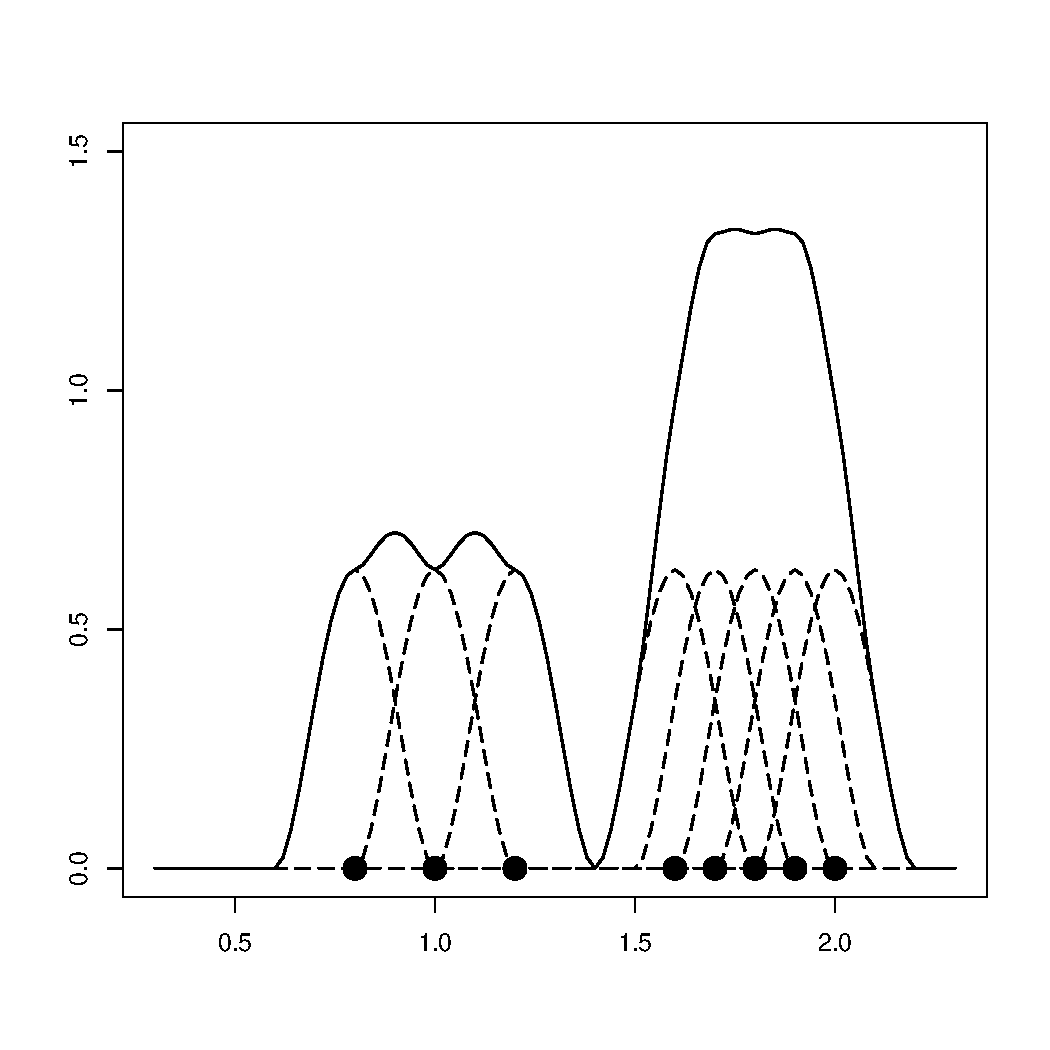
\includegraphics[width=\textwidth]{img/kernel1d-02}
        \subcaption{$h=0.2$}
        \label{fig:theory:kernel1d:02}
    \end{subfigure}
    \begin{subfigure}[t]{0.32\textwidth}
        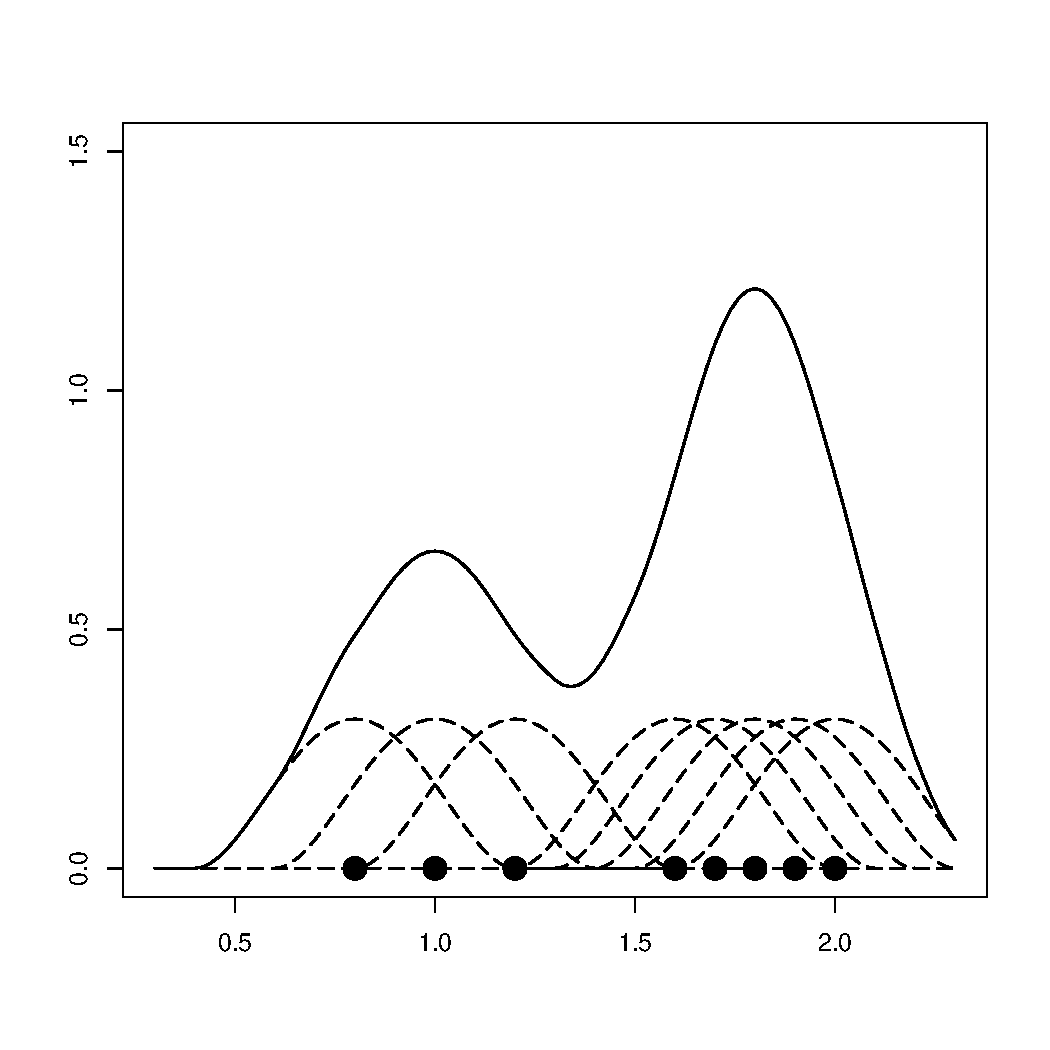
\includegraphics[width=\textwidth]{img/kernel1d-04}
        \subcaption{$h=0.4$}
        \label{fig:theory:kernel1d:04}
    \end{subfigure}
    \begin{subfigure}[t]{0.32\textwidth}
        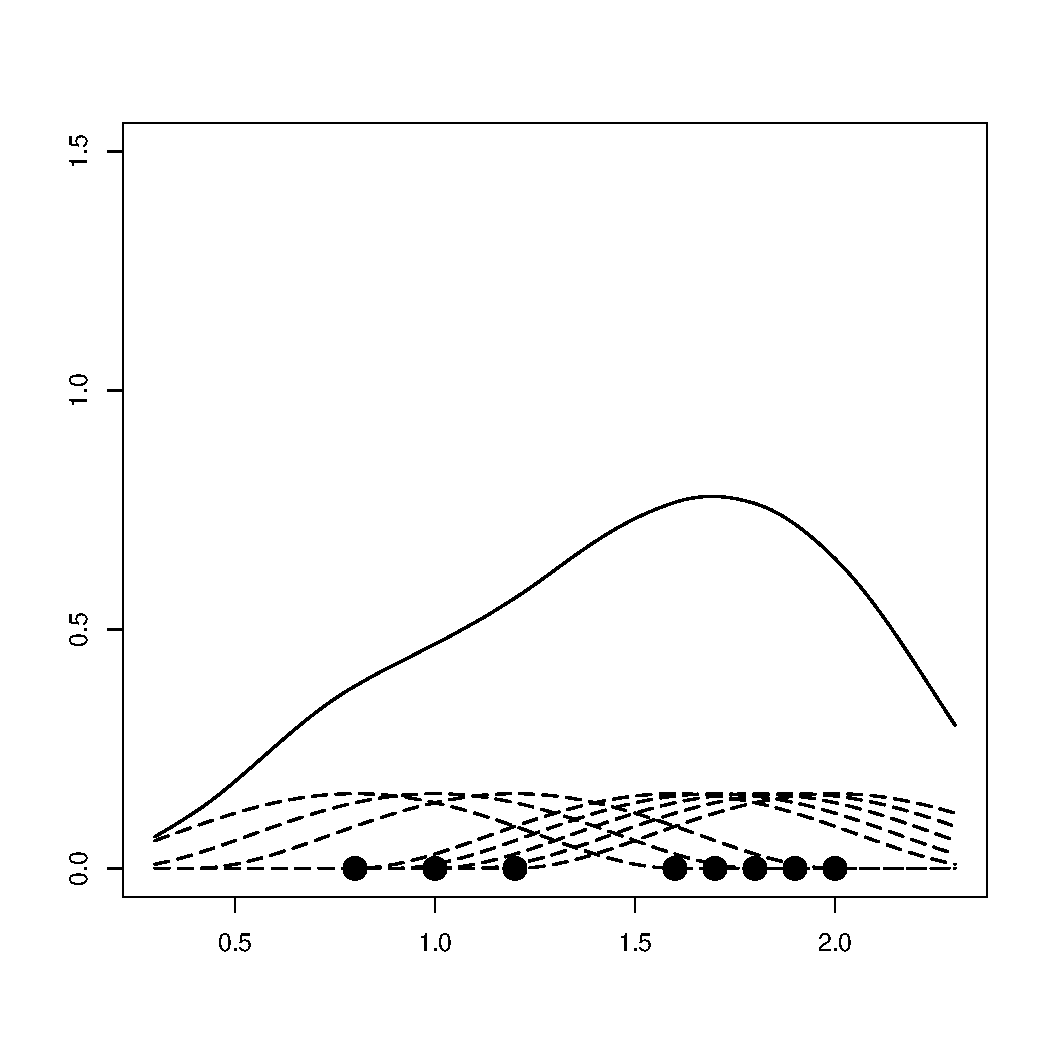
\includegraphics[width=\textwidth]{img/kernel1d-08}
        \subcaption{$h=0.8$}
        \label{fig:theory:kernel1d:08}
    \end{subfigure}
    \caption[One-dimensional \glsentryname{kernel} functions]
        {One-dimensional \glsentryname{kernel} functions using the biweight(quartic) kernel \citep{silverman1986density}.
        The dots on the $x_1$ axis are the observed \glsentryplural{event}.
        The dashed lines are the kernel functions around these \glsentryplural{event}
        and the solid line is the \glsentryname{intensity} estimate $\hat{\lambda_1}$.}
    \label{fig:theory:kernel1d}
\end{figure}

\Cref{fig:theory:kernel1d} shows an example of how \gls{kernel} smoothing works in  one-dimension for three different bandwidths.
The dots along the bottom are the observed \glspl{event}.
The dashed lines show the \gls{kernel} functions around each of these \glspl{event},
while the upper solid line is the \gls{intensity} estimate produced using \Cref{eq:lambda_hat_1}.
\Cref{fig:theory:kernel1d:02} shows the estimate with $h=0.2$.
It has two local modes, each with a bit of fluctuation at the peaks.
In \Cref{fig:theory:kernel1d:04} we still see two modes with $h=0.4$, but with smoother peaks.
\Cref{fig:theory:kernel1d:08} has smoothed the two peaks together into a single,
large peak by using the larger bandwidth of $h=0.8$.

The two-dimensional case is analogous.
Starting with a set of \glspl{event} $\gls{N} \subset \RS$,
and a positive value \gls{h} known as the bandwidth,
we define the the \gls{kernel intensity estimator} as follows:
\begin{defn}
    \label{defn:lambda_hat}
    The \textbf{\gls{kernel intensity estimator}} $\gls{lambda_hat}_h \xvec$
    is a technique for estimating the \gls{intensity} of an \gls{spp}
    from observed \glspl{event} \gls{N}.
    The formula for computing the \gls{kernel intensity estimator} is:
    \begin{equation}
        \label{eq:lambda_hat}
        \gls{lambda_hat}_h \xvec%
            = \sumS{\gls{K}\left( \frac{\xvec-(s_1, s_2)}{h} \right)} \text{.}%
    \end{equation}
\end{defn}
where $\xvec-(s_1, s_2)$ is ordinary vector subtraction,
and $\frac{\xvec-(s_1, s_2)}{h}$ is scalar multiplication by $\frac{1}{h}$.
For the remainder of this section we treat $h$ as a scalar for ease of explanation.
However, with no loss of generality we will use separate bandwidths in each coordinate,
that is $\mathbf{h}=(h_1, h_2)$.

There are many kernels which satisfy \Cref{eq:k_pos,eq:k_1},
including two-dimensional versions of the square kernel, the Gaussian kernel and the Epanechnikov kernel.
In this study we use the two-dimensional biweight kernel,
also known as the quartic kernel,
which can be found in \citet{silverman1986density} with formula
\begin{equation}
    \label{eq:biweightkernel2d}
    K \xvec =%
    \begin{cases}%
        \frac{3}{\pi}\left( 1 - x_1^2 - x_2^2 \right)^2 & \text{if}~x_1^2+x_2^2<1 \\%
        0 & \text{otherwise.}%
    \end{cases}%
\end{equation}
This kernel spreads the weight of each event \xvec~ into a circle of radius one, centered at \xvec.
The effect of the bandwidth $h$ is to change the radius of that circle to $h$.
The advantage of the kernels over the Epanechnikov kernel is that it twice-differentiable.
The advantage over the Gaussian kernel is that it much faster to compute.

%%%%%%%%%%%%%%%%%%%%%%%%%%%%%%%%%%%%%%%%%%%%%%%%%%%%%%%%%%%%%%%%%%%%%%%%%%%%%%
%%
%% Kernel density estimation
%%
%%%%%%%%%%%%%%%%%%%%%%%%%%%%%%%%%%%%%%%%%%%%%%%%%%%%%%%%%%%%%%%%%%%%%%%%%%%%%%
\section{Kernel density estimation}
 
While there is some theoretical work available for \gls{kernel intensity estimation},
it is usually based on and compared to \acrfull{kde}.
\Gls{kde} is a popular method of non-parametric estimation of probability density functions from observed data.

The primary reference for probability density estimation is \citet{silverman1986density},
which covers both parametric and non-parametric methods.
In particular,
he covers kernel methods,
including the multi-dimensional \gls{kernel intensity estimation} used in this research.
We note that both of our bandwidth selection methods,
the \Gls{silverman} Rule of Thumb and the least-squares \acrlong{cv} are discussed in this book.
The earliest paper to discuss \gls{kde} for probability density functions was by \citet{rosenblatt1956remarks}.
It contains derivations of the bias, variance,
and \acrfull{mise} for general density estimates in one dimension,
and introduces the class of kernel estimates.
\Citet{wand1993comparison} take an in-depth look at smoothing parameters in two dimensions.
In particular,
they find that using a two-dimensional bandwidth vector is adequate for smoothing in each coordinate direction.
In another book, \citet{wand1994kernel}
give a broad overview of kernel methods,
including several techniques for selecting the bandwidth.
In examining how both the \gls{kde} and \gls{kernel intensity estimation} can use data to learn about underlying structure,
they describe how these similar techniques are used in comparison to parametric methods.
In addition to single and multi-variable kernel methods to estimate functions,
they also describe how kernel regression techniques can be used for supervised learning and prediction.

A different perspective can be found in \citet{devroye1985nonparametric},
which analyses non-parametric density estimation from an $L_1$ perspective,
which is in line with our use of the \gls{miae} measure of accuracy.

%%%%%%%%%%%%%%%%%%%%%%%%%%%%%%%%%%%%%%%%%%%%%%%%%%%%%%%%%%%%%%%%%%%%%%%%%%%%%%
%%
%% Measuring the accuracy of the estimate
%%
%%%%%%%%%%%%%%%%%%%%%%%%%%%%%%%%%%%%%%%%%%%%%%%%%%%%%%%%%%%%%%%%%%%%%%%%%%%%%%%
\section{Measuring the accuracy of the estimate}
\label{sec:theory:accuracy}

This section is based on \citet{silverman1986density} and \citet{wand1994kernel}.
A common statistical problem is to find the ``best'' estimate \gls{lambda_hat}
for the \gls{intensity} of an unknown \gls{spp}
based on a set of observed \glspl{event}.
In order to do this using \gls{kernel intensity estimation},
we must select the ``best'' bandwidth.
From \Cref{fig:theory:kernel1d} we can see that different values of bandwidth \gls{h} result in different estimates for the \gls{intensity}.
Our goal is to find a decision procedure that gives us the ``best'' result.
While there is a great deal of research in \gls{kde},
there is much less work available for \gls{kernel intensity estimation}.
We make use of one such result:
the optimal bandwidth used for computing the \gls{kernel intensity estimator} is the same as that for computing the related \gls{kde} function,
and can be determined by the same techniques \Citep{diggle1988equivalence}.
However, the \gls{kde} is used to estimate a probability density function,
while the \gls{kernel intensity estimator} is used to compute an intensity function.
Computationally, the difference is that a density must integrate to one,
and in order to do that,
we divide by $n$,
the number of observed events.


The first thing we must do is define what we mean by the ``best'' result.
We do this by choosing a measure of accuracy for the estimate,
and selecting the bandwidth which gives the optimal value for this measure.
One common accuracy measure used for function estimation is the \gls{mise},
because it has several useful mathematical properties.
It allows for additional analysis by being broken down into the mean integrated squared bias and mean integrated variance.
It can also be estimated by \acrlong{cv}.

Given a realized estimate \gls{lambda_hat} for any function \gls{lambda},
we can compute the squared error at any given point $\xvec \in \RS$ as
$\left( \lmbdhat - \lmbd \right)^2$,
and its expected value at $\xvec$ is called the \gls{mse}.
However,
we would like to compute the accuracy of the whole function.
We do this by integrating the squared error of the estimate over the study area to obtain the \gls{ise}.
\begin{equation}
\label{eq:ise}
    \mbox{\gls{ise}}(\gls{lambda_hat}) = \iintW{
            \left( \lmbdhat - \lmbd \right)^2
    }
\end{equation}
The \gls{mise} is the expected value of the \gls{ise} over the sample space of realizations of \gls{Lambda}.
\begin{align}
    \mbox{\gls{mise}}(\gls{lambda_hat}) 
        & = \E [\mbox{\gls{ise}}(\gls{lambda_hat})] \nonumber \\
        & = \E \iintW{ \left( \lmbdhat - \lmbd \right)^2 } \label{eq:mise}
\end{align}
The integrand of \Cref{eq:mise} is non-negative.
Therefore, by Fubini's Theorem, we can change the order of integration and expectation.
\begin{align}
    \mbox{\gls{mise}}(\gls{lambda_hat}) 
        & = \iintW{ \E \left( \lmbdhat - \lmbd \right)^2 } \nonumber \\
        & = \iintW{ \mbox{\gls{mse}}(\gls{lambda_hat}, \xvec) } \nonumber
\end{align}

We decompose \gls{mse} into the squared bias and squared variance% (\Cref{eq:mse:biasvariance}),
giving us
\begin{align}
    \mbox{\gls{mise}}(\gls{lambda_hat}) 
        & = \iintW{ \Big( \E\lmbdhat - \lmbd \Big)^2 } \nonumber \\
        & \qquad + \iintW{ \E \Big( \lmbdhat - \E\lmbdhat \Big)^2 } \label{eq:mise:intbiasvariance}
\end{align}
We call the first part of \Cref{eq:mise:intbiasvariance} the \gls{isb} and the second part the \gls{iv}.

%%%%%%%%%%%%%%%%%%%%%%%%%%%%%%%%%%%%%%%%%%%%%%%%%%%%%%%%%%%%%%%%%%%%%%%%%%%%%%
%%
%% Asymptotic behavior of the bandwidth
%%
%%%%%%%%%%%%%%%%%%%%%%%%%%%%%%%%%%%%%%%%%%%%%%%%%%%%%%%%%%%%%%%%%%%%%%%%%%%%%%
\section{Asymptotic behavior}
\label{sec:theory:asymptotic_bandwidth}

For the \gls{kernel intensity estimator},
the \gls{mise} cannot be computed directly.
Instead,
we need to approximate it.
In order to do this,
we compute approximate values of the bias,
the variance,
and finally we can compute the \gls{amise} which is the sum of the approximate variance and the square of the approximate bias.
This allows us to analyze the behavior of the \gls{mise} asymptotically,
with dependence only on the true function $\gls{lambda}\dotdot$ and the kernel $K\dotdot$.

Following \citep{silverman1986density,wand1994kernel},
and based on the equivalence of bandwidths for the \gls{kde} and the\gls{kernel intensity estimator} \citep{diggle1988equivalence},
we begin by using Taylor's Theorem to approximate the \gls{kde}.
Let \gls{f} be a probability density function,
and define the \gls{kde} of \gls{f}:
\begin{equation}
    \gls{f_hat} \xvec%
            = \sumSn{\gls{K}\left( \frac{\xvec-(s_1, s_2)}{h} \right)} \text{.}%
\end{equation}
We make the following assumptions about $K\dotdot$
and $f\dotdot$ \citep{silverman1986density,wand1994kernel}:
\begin{assumptions}
    \item $K\dotdot$ is a probability density function with zero mean \label{amise:assumptions:1}
    \item $K\dotdot$ is radially symmetric and has non-zero, finite variance \label{amise:assumptions:2}
    \item $f\dotdot$ has bounded and continuous second derivatives. \label{amise:assumptions:3}
\end{assumptions}

Under these assumptions,
the first term of the Taylor expansion is zero (\cref{amise:assumptions:1,amise:assumptions:3}),
and the second and remainder terms of the Taylor expansion are finite (\cref{amise:assumptions:2}).
The following formulas for the \gls{amise} can be found it \citet[Section 4.3]{silverman1986density}.
\begin{align}
    \mbox{bias}_h \hat{f} \xvec%
        & \approx \frac{1}{2} h^{2} \alpha \nabla^2 f \xvec \nonumber \\%
    \mbox{variance}_h \hat{f} \xvec%
        & \approx n^{-1} h^{-2} \beta f \xvec \nonumber \\%
    \mbox{\gls{amise}}(f; h)%
        & = \frac{1}{4} h^{4} \alpha^2 \iintW{\left( \nabla^2 f \xvec \right)^2 }%
            + n^{-1} h^{-2} \beta \label{eq:amisef}%
\end{align}
where
\begin{align}
    \alpha & = \iintR{x_1^2 K(x_1,x_2)} \text{, since}~K\dotdot~\text{is radially symmetric,} \nonumber \\
    \beta & = \iintR{\Big( K(x_1,x_2) \Big)^2} \text{, and} \nonumber \\
    \nabla^2 f \xvec & = \frac{\diffsq{f}\xvec}{\diff{x_1^2}} + \frac{\diffsq{f}\xvec}{\diff{x_2^2}} \nonumber \text{.}
\end{align}

We note that both $\alpha$ and $\beta$ depend only on \Kdots,
and that $\nabla^2 f$ is the Laplacian operator which is the trace of the Hessian matrix.
We can now take the derivative of \Cref{eq:amisef} by $h$ and set it to zero,
giving us the optimal bandwidth \gls{h_opt}:
\begin{align}
    \gls{h_opt} & = C n^{-\frac{1}{6}}
\end{align}
where $C$ is a constant that depends on $\lambda$ and $K$.
\begin{defn}
    The \gls{mise} \textbf{optimal bandwidth} $\mathbf{\gls{h_opt}}$ is the value of $h$ that minimizes the \gls{mise} of the \gls{kde} for a given probability density function $f$ and kernel function $K$.
\end{defn}
As noted above,
the optimal bandwidth of the \gls{kde} in the \gls{mise} sense is the same for the \gls{kernel intensity estimator}.
For $h < \gls{h_opt}$, the variance will be higher, while $h > \gls{h_opt}$ will result in a higher bias \Citep{rosenblatt1971curve}.

Since we have $\gls{lambda_hat} = n \hat{f}$,
the formula for the \gls{amise} of $\gls{lambda} = \mu f$ is
\begin{align}
    \mbox{bias}_h \gls{lambda_hat} \xvec%
        & \approx \frac{1}{2} h^{2} \alpha \mu \nabla^2 f \xvec \nonumber \\%
    \mbox{variance}_h  \gls{lambda_hat} \xvec%
        & \approx n^{-1} h^{-2} \beta \mu f \xvec \nonumber \\%
    \mbox{\gls{amise}}(\gls{lambda}; h)%
        & = \frac{1}{4} h^{4} \alpha^2 \mu^2 \iintW{\left( \nabla^2 f \xvec \right)^2 }%
            + \mu^2 n^{-1} h^{-2} \beta \label{eq:amiselambda}%
\end{align}

There are other accuracy measures that can be used to evaluate the estimate of the \gls{kernel intensity estimator}.
We discuss some of these in \Cref{sec:method:accuracy}.
Although we use these measures to characterize the behavior of the \gls{kernel intensity estimator} and the \gls{dkd},
our bandwidth is chosen by techniques that try to achieve \gls{h_opt} and minimize \gls{mise}.
However, as noted above,
our approximation \gls{amise} depends on the true risk function \gls{lambda}.


%%%%%%%%%%%%%%%%%%%%%%%%%%%%%%%%%%%%%%%%%%%%%%%%%%%%%%%%%%%%%%%%%%%%%%%%%%%%%%
%%
%% Bandwidth selection from data
%%
%%%%%%%%%%%%%%%%%%%%%%%%%%%%%%%%%%%%%%%%%%%%%%%%%%%%%%%%%%%%%%%%%%%%%%%%%%%%%%
\section{Bandwidth selection from data}
\label{sec:theory:bandwidthselection}

In practice,
researchers typically do not know the true density or intensity functions.
Therefore they cannot compute \gls{h_opt} directly,
and so they use techniques that give them approximations for this value.
In this study,
we do know the true intensity functions,
since we use them to generate data for the simulations.
Therefore we can compute the ``best'' bandwidth by comparing to the actual truth.
We therefore define
\begin{defn}
    the \textbf{\gls{oracle bandwidth}} for a given \gls{intensity} is the bandwidth that minimizes the empirical \gls{mise},
    computed from the data samples generated from the true \gls{intensity} function.
\end{defn}
Other schemes for selecting the bandwidth that are based on a specific data sample will not be as good as the \gls{oracle}.
The two techniques we use are optimized to find a bandwidth that minimizes \gls{mise}.
The selected bandwidth may or may not be close to \gls{h_opt},
depending on the particular sample.
The first technique we will use is known as \textbf{\Gls{silverman}'s Rule of Thumb}.
We use the version for selecting bandwidth in $\RS$,
which has forumula
\begin{equation}
    \label{eq:silverman}
    h_S = 2.04 * \sigma * n^{-1/6}%
\end{equation}
where $n$ is the observed number of incidents,
$\sigma$ the arithmetic mean of $\sigma_{x_1}$ and $\sigma_{x_2}$,
he standard deviations of the $x_1$ and $x_2$ coordinates of the sample points respectively:
\begin{equation}
    \sigma = \frac{\sigma_{x_1} + \sigma_{x_1}}{2} \text{.}
\end{equation}
\citet{silverman1986density} shows that for a large class of intensity functions,
including ones based on Gaussian functions,
this bandwidth provides a good approximation to the optimal bandwidth \gls{h_opt}. 

Our second technique is to use leave-one-out \textbf{\gls{cv}} over a set of bandwidths.
We select the bandwidth which minimizes the \gls{cv} error,
which approximates the \gls{mise} (\Cref{eq:mise}).
For the \gls{kde},
he formula for the \gls{cv} error of bandwidth $h$ for \gls{lambda_hat} is
\begin{equation}
    \label{eq:cverror}
    \mbox{\Gls{cv}}%
        = \iintW{\gls{lambda_hat}_h \xvec^2}
        - 2 n^{-1} \sum\limits_{i=1}^n \gls{lambda_hat}_{-i,h}\xvec%
\end{equation}
where $\gls{lambda_hat}_{-i,h}\xvec$ is the \gls{kernel intensity estimator} computed using the bandwidth $h$ and leaving out the $i^\text{th}$ point.
The technique for \gls{kernel intensity estimation} is identical to the \gls{kde},
in the sense that the bandwidths which minimize the \gls{mise} of the \gls{kernel intensity estimator} are the same \citep{brooks1991asymptotic}. 
\Citet{brooks1991asymptotic} show that the \gls{cv} error computed with the selected bandwidth approximates the optimal \gls{ise} very well,
in the sense that
\begin{equation}
    \frac   {\mbox{\gls{ise}}(\gls{lambda_hat}; h_{\gls{cv}})}%
            {\mbox{\gls{ise}}(\gls{lambda_hat}; \gls{h_opt})}%
            \to 1 ~\text{almost surely.}%
\end{equation}

%%%%%%%%%%%%%%%%%%%%%%%%%%%%%%%%%%%%%%%%%%%%%%%%%%%%%%%%%%%%%%%%%%%%%%%%%%%%%%
%%
%% Inconsistency of the kernel intensity estimator
%%
%%%%%%%%%%%%%%%%%%%%%%%%%%%%%%%%%%%%%%%%%%%%%%%%%%%%%%%%%%%%%%%%%%%%%%%%%%%%%%
\section{Inconsistency of the kernel intensity estimator}
\label{sec:theory:inconsistency}

The \gls{kde} $\hat{f}$ can be shown to be a consistent estimator of a density function $f$.
\citet{bertrand1978convergence} show that the \gls{kde} converges uniformly to the true function with probability 1 as $n \to \infty$,
while \citet{devroye1985nonparametric} show that the \gls{kde} converges in $L_1$ to the true function with probability 1.
In contrast to density functions,
where the estimate is normalized by the number of observations,
for a spatial intensity
both the magnitude of the scaling factor \gls{mu} of the true intensity
and the number of observed events $n$ are proportional
to both the time frame of the study or the size of the study area.
Therefore,
in order to discuss the asymptotic behavior of an intensity function,
it makes sense to look at $\gls{mu} \to \infty$.
We describe the behaviour of the \gls{dkd} as \gls{mu} increases in \Cref{sec:results:unifNpop_1h}.
Along these lines,
\citet{guan2008consistent} note that the \gls{kernel intensity estimator}
``is not a consistent estimator of the true intensity''.

We therefore \textit{normalize} our measures of accuracy in two ways.
The first way is to simply divide our approximated \gls{mise} by $\gls{mu}^2$
as suggested by \citet{diggle1988equivalence},
since we know the true function and therefore \gls{mu}.
The second way is to divide, at every point,
the estimation error $\gls{lambda_hat}\xvec - \gls{lambda}\xvec$ by the true value $\gls{lambda}\xvec$.
Our results contain these and similar relative errors for all of the accuracy measures
as described in \Cref{sec:method:accuracy}.

%%%%%%%%%%%%%%%%%%%%%%%%%%%%%%%%%%%%%%%%%%%%%%%%%%%%%%%%%%%%%%%%%%%%%%%%%%%%%%
%%
%% Kernel intensity estimation
%%
%%%%%%%%%%%%%%%%%%%%%%%%%%%%%%%%%%%%%%%%%%%%%%%%%%%%%%%%%%%%%%%%%%%%%%%%%%%%%%
\section{Kernel intensity estimation}

The idea to use \gls{kernel intensity estimation} to estimate the intensity functions of one-dimensional point processes can be found in \citet{diggle1985kernel}.
Based on the kernel methods described by \citet{rosenblatt1956remarks},
and making use of edge-correction,
Diggle's paper includes estimates for the \gls{mise} as well as a performance evaluation using simulated data.
The equivalence of the bandwidth in kernel density and intensity was shown in \citet{diggle1988equivalence}.
\Citet{brooks1991asymptotic} show that the \gls{cv} bandwidth is asymptotically optimal,
building on similar results for the \gls{kde} \citep{hall1983large,burman1985data,stone1984asymptotically}.

% Unlike the \gls{kde} however,
% the \gls{kernel intensity estimator} is not consistent,
% meaning that the \gls{mise} does not converge to zero as the number of incidents increases.
% There is some work in this area,
% with \citet{guan2008consistent} and \citet{fuentes2016consistent} developing techniques for \gls{kernel intensity estimation} that are consistent under certain conditions.
% The research mentioned above is mostly concerned with one-dimensional data.
% However, kernel technieques have successfully been used in two dimensions as well \citep{scott1992multivariate}.

%%%%%%%%%%%%%%%%%%%%%%%%%%%%%%%%%%%%%%%%%%%%%%%%%%%%%%%%%%%%%%%%%%%%%%%%%%%%%%
%%
%% Application to epidemiology
%%
%%%%%%%%%%%%%%%%%%%%%%%%%%%%%%%%%%%%%%%%%%%%%%%%%%%%%%%%%%%%%%%%%%%%%%%%%%%%%%
\section{Application to epidemiology}

Current research in kernel estimation continues.
For example, we see kernel estimation techniques used in epidemiology.
Like our research,
the tutorial paper \citet{davies2018tutorial} looks at using the ratio of two kernel estimates for estimating epidemiological risk functions.
However,
they also delve into several additional bandwidth selection techniques,
edge corrections,
and other methods that extend the basic \gls{kde}.
Their paper is based on the technique developed by \citet{bithell1990application,bithell1991estimation,kelsall1995kernel}.
By conditioning on sample size,
they compute two \glspl{kde} instead of \glspl{kernel intensity estimator} in order to compare the relative risk between two samples representing the case and control populations on a common study area.
This relative risk ratio represents a different quantity from the incidence rate of our current research.

In many studies,
incidents of disease are aggregated together instead of using spatial analysis.
This is referred to as ``zonal analysis'' and suffers from several issues,
mainly due to information that is lost when aggregating and computing \glspl{asr}.
One of the motivations of spatial analysis is to provide more informative results than can be done with aggregation.
An example of how the results of studies based on such aggregation can be misleading can be found in \citet{portnov2007ecological}.

%%%%%%%%%%%%%%%%%%%%%%%%%%%%%%%%%%%%%%%%%%%%%%%%%%%%%%%%%%%%%%%%%%%%%%%%%%%%%%
%%
%% The double kernel
%%
%%%%%%%%%%%%%%%%%%%%%%%%%%%%%%%%%%%%%%%%%%%%%%%%%%%%%%%%%%%%%%%%%%%%%%%%%%%%%%
\section{The double kernel}

The \acrfull{dkd} has been used in epidemiological studies since at least 2004 \citep{rushton2004analyzing}.
\citet{kloog2009using} is another recent study which uses the \gls{dkd}.
In particular,\
it identifies the \gls{maup},
which occurs when changes to the arbitrary administration zones that are used to aggregate incidents can result in different observations and findings.
\citet{zusman2012residential} is another study which discusses the advantages of the \gls{dkd} over \glspl{asr}.
A recent examination of the properties of the \gls{dkd} can be found in \citet{zusman2016application}.
They find that:
\begin{quotation}
The DKD approach provides reasonably stable and consistent estimates, if the following three preconditions are met: (a) the kernel estimation parameters are properly defined, (b) the number of reference points, used for transformation of continuous DKD surfaces into discrete observations, is sufficiently large, and (c) the spatial dependency of neighboring observations is taken into account.
\end{quotation}

%%%%%%%%%%%%%%%%%%%%%%%%%%%%%%%%%%%%%%%%%%%%%%%%%%%%%%%%%%%%%%%%%%%%%%%%%%%%%%
%%
%% Data generation process
%%
%%%%%%%%%%%%%%%%%%%%%%%%%%%%%%%%%%%%%%%%%%%%%%%%%%%%%%%%%%%%%%%%%%%%%%%%%%%%%%
\section{Data generation process}
\label{sec:theory:data}

We generate data for each experiment using rejection sampling,
based on the technique suggested in \Citet[Section 4.4]{diggle1983spatial},
based on \citet{lewis1979simulation}.
However,
because we are dealing with a \textit{rate} that affects members of a \textit{population},
our algorithm is slightly different.
To be more specific,
the algorithm mentioned in the aforementioned book consists of simulating a Poisson process on \gls{W}
with intensity $\lambda_0$ equal to the maximum value of $\gls{lambda}(x_1, x_2)$ within \gls{W},
and retaining an event at $(x_1, x_2)$ with
probability $\gls{lambda}(x_1, x_2)/\lambda_0$.
Our data generation algorithm differs from the one suggested by \citet{lewis1979simulation} in the following way.
In our case,
we are interested in both the \glspl{incident} and the population as a whole.
We therefore first generate a population according to our chosen population distribution,
and apply the \gls{incident} rate function to each ``person'' to determine which ones ``fell ill''.

Essentially, their algorithm chooses $N_p$ points at random in \gls{W}.
Our algorithm uses a fixed set of $N_p$ points, generated one time per experiment according to the chosen population distribution.
Both algorithms apply \gls{lambda} to the ``persons'' in order to generate incidents.

We proceed in two parts.
First, we generate a population \gls{P} of the chosen size $N_p$ as follows:
\begin{itemize}
    \item If the population is to be uniform,
            we choose $N_p$ points uniformly in \gls{W}.
        so that we generate the desired population count $N_p$.
    \item If the population is to be peaked,
            we choose $N_p$ points from a bivariate normal distribution,
            centered at $(c_1, c_2)$,
            with covariance matrix
            $\begin{pmatrix}
                \sigma_1 & 0 \\
                0 & \sigma_2
            \end{pmatrix}$.
            In practice, we use the same value for $\sigma_1$ and $\sigma_2$.
\end{itemize}

This population is a simulated set of \glspl{event} from our chosen population \gls{spp}.
Once we have a population,
we can repeatedly simulate sample sets of \glspl{incident} using the following procedure:
\begin{enumerate}
    \item We create the risk function \gls{lambda}
        by scaling a basic \gls{intensity} function $f$ of the desired shape.
        The meaning of $f$ being an \gls{incidence rate} is that for given a ``person'' $(p_1, p_2) \in \gls{P}$,
        an incident occurring at $(p_1, p_2)$ is a Bernoulli random variable with probability $f(p_1, p_2)$.
        Therefore the expected number of \glspl{incident} at $(p_1, p_2)$ is $f(p_1, p_2)$.
        We compute $f(x_1, x_2)$ across a grid of points in \gls{W} and take the mean,
        giving us
        $$
            \mu_f = \mean\limits_{(p_1, p_2) \in P}{f(p_1,p_2)} \text{,}
        $$
        the expected number of \glspl{incident} generated by $f$ for a single, randomly generated point in \gls{W}.
        When we multiply $N_p \times \mu_f$,
        we get the expected number of \glspl{incident} generated by $f$
        for a uniformly distributed population of size $N_p$.
        So, if we take a uniformly distributed population \gls{P} of size $N_p$,
        and apply $\frac{1}{N_P \times \mu_f} f$ to each point $(p_1, p_2) \in \gls{P}$,
        the expected number of \glspl{incident} is 1.
        Therefore, if our desired expected number of \glspl{incident} for a uniform population of size $N_p$
        under rate \gls{lambda} is $N_i$,
        we must compute \gls{lambda} by scaling $f$ using the following formula:
        $$
            \gls{lambda}(p_1, p_2) = \frac{N_i}{N_p \times \mu_f} f(p_1, p_2)\text{.}
        $$
    \item For each ``person'' $p\!=\!(p_1, p_2) \in \gls{P}$,
        we calculate the \textit{risk} of coming down with the disease $\gls{lambda}(p_1, p_2)$
    \item Keep $(p_1, p_2)$ in \gls{I} with probability $\gls{lambda}(p_1, p_2)$.
\end{enumerate}

In this way,
when the population is uniformly distributed,
the expected value of the number of \glspl{incident} is $N_i$.
In cases where the population has a peak,
the risk function \gls{lambda}\dotdot is still the same,
but the expected number of \glspl{event} is not necessarily $N_i$.
This allows us to compare different population distributions for the same risk function.

Due to the large size of the population,
we use the same \textbf{fixed} population \gls{P} for an entire experiment
in order to perform the experiments in a reasonable amount of time.
Therefore,
we do not study the randomness in the population distribution in this study.

Our $\gls{lambda}(x_1, x_2) \leq 1$ is a probability at every $(x_1, x_2) \in \gls{W}$,
so the number of \glspl{incident} follow a Poisson-Binomial distribution which,
according to Le Cam's Theorem, approximates the Poisson Distribution.
Therefore, this method that generates \glspl{incident} approximates an Inhomogeneous Poisson Process,
with mean $\sum\limits_{i=1}^{N_p}{\frac{N_i}{N_p \times \mu_f} f(p_{i1}, p_{i2})} = N_i$.

While the \gls{dkd} has been used frequently in epidemiological and non-epidemiological spatial analysis,
its statistical properties have not been adequately studied.
In order to understand these properties,
both a theoretical and an empirical analysis is required.
The scope of this research is to provide a beginning to the empirical analysis by studying the sensitivity of the \gls{dkd} to several factors using monte carlo simulations.

